\documentclass{beamer}
\usetheme{Boadilla}
\usecolortheme{whale}
\usepackage{comment}
\usepackage{ragged2e}
\usepackage{amsmath}
\usepackage{dcolumn}
\usepackage{booktabs}
\usepackage{pdflscape}
\usepackage{graphicx}
\usepackage{placeins}
\usepackage{dcolumn}
\usepackage{xcolor}
\usepackage{booktabs}
\linespread{1.5}
\usepackage{subcaption}
\usepackage{amsmath}
\usepackage{hyperref}
\usepackage{multirow}
\usepackage{tikz}
\usepackage[title]{appendix}
\usetikzlibrary{decorations.pathreplacing}
\usepackage{booktabs}
\usepackage{tabularx}
\usepackage{datatool}

%\usepackage{xepersian}
%\settextfont{XB Zar}
%\setdigitfont{XB Zar}


\renewcommand{\today}{\ifcase \month \or January\or February\or March\or %
April\or May \or June\or July\or August\or September\or October\or November\or %
December\fi, \number \year} 


\AtBeginSection[]
{
    \begin{frame}
        \frametitle{Table of Contents}
        \tableofcontents[currentsection]
    \end{frame}
}

\title[Speculative Betas]{Speculative Betas\footnote{ \tiny Jornal of Finance - 2016}}
\subtitle{Harrison Hong \qquad David A.Sraer}
\author[Aghajanzadeh]{S.M. Aghajanzadeh  }
\institute[]{Tehran Institute for Advanced Studies }
\centering

\begin{document}

{\maketitle}
\small

\begin{frame}{$ \beta $-Sorted Portfolios}
	\begin{itemize}
		\item At the beginning of each calendar month, stocks are ranked in ascending order on the basis of their estimated beta at the end of the previous month for prior year
		\item The ranked stocks are assigned to 1 of 20 value-weighted portfolios
	\end{itemize}
	\begin{figure}
		\centering
		\includegraphics[width=0.9\linewidth]{"../Paper Presentaion/t1"}
	\end{figure}
\end{frame}



\begin{frame}{Iran $ \beta $-Sorted Portfolios}
	\begin{itemize}
	\item At the beginning of each calendar month, stocks are ranked in ascending order on the basis of their estimated beta at the end of the previous month for prior year
	\item The ranked stocks are assigned to 1 of 10 market-weighted portfolios
\end{itemize}	
	\begin{table}[htbp]
		\centering
		\resizebox{0.9\textwidth}{!}{
			\begin{tabular}{lrrrrrrrrrr}
	\toprule
	Portfolio & 1     & 2     & 3     & 4     & 5     & 6     & 7     & 8     & 9     & 10 \\
	\hline
	$ \beta $ & 0.64  & 0.68  & 0.71  & 0.82  & 0.96  & 1.21  & 1.13  & 1.26  & 1.38  & 1.77 \\
	12Return & 16.63 & 29.71 & 26.14 & 32.11 & 33.24 & 34.16 & 32.44 & 30.58 & 37.38 & 39.75 \\
	Mreturn & 1.73  & 2.47  & 2.32  & 2.76  & 3.38  & 2.69  & 2.91  & 2.53  & 3.43  & 3.67 \\
	Size  & 35    & 36    & 37    & 37    & 37    & 38    & 38    & 38    & 38    & 36 \\
	\bottomrule
	
	
\end{tabular}
			\label{tab:addlabel}	
		}
	\end{table}
\end{frame}
\begin{frame}{Beta and Return}
	\begin{figure}
		\centering
		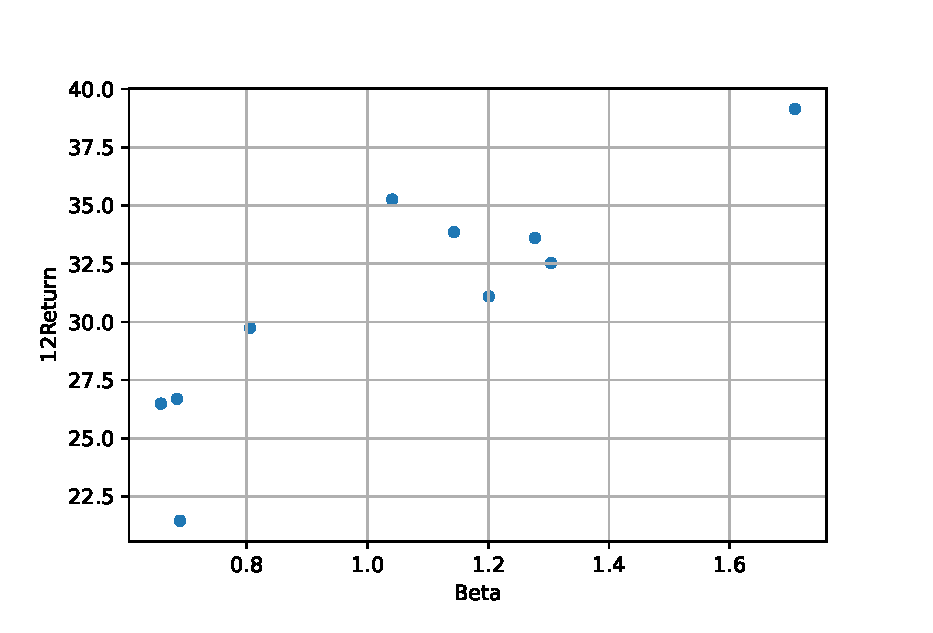
\includegraphics[width=0.7\linewidth]{BetaReturn10.eps}
		\label{fig:BetaReturn}
	\end{figure}
	
\end{frame}

\begin{frame}{Beta and Return}
	\begin{figure}
		\centering
		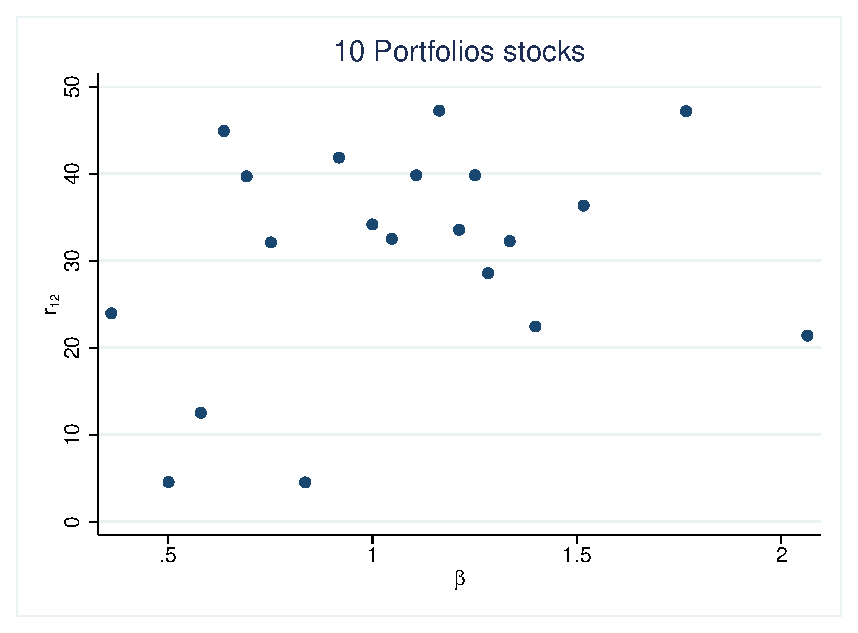
\includegraphics[width=0.7\linewidth]{10portfo.eps}
		\label{fig:betareturn}
	\end{figure}
	
\end{frame}


\begin{frame}{$ \beta $-Sorted Portfolios}
	\begin{itemize}
		\item Rank stocks based on preranking ratio of $ \beta $ to $ \sigma^2 $ and define as speculative stocks all stocks with a ratio above  the  median ratio
		\item Then, within each of these two groups creat 20 $ \beta $-sorted portfolios
	\end{itemize}
	\begin{figure}
		\centering
		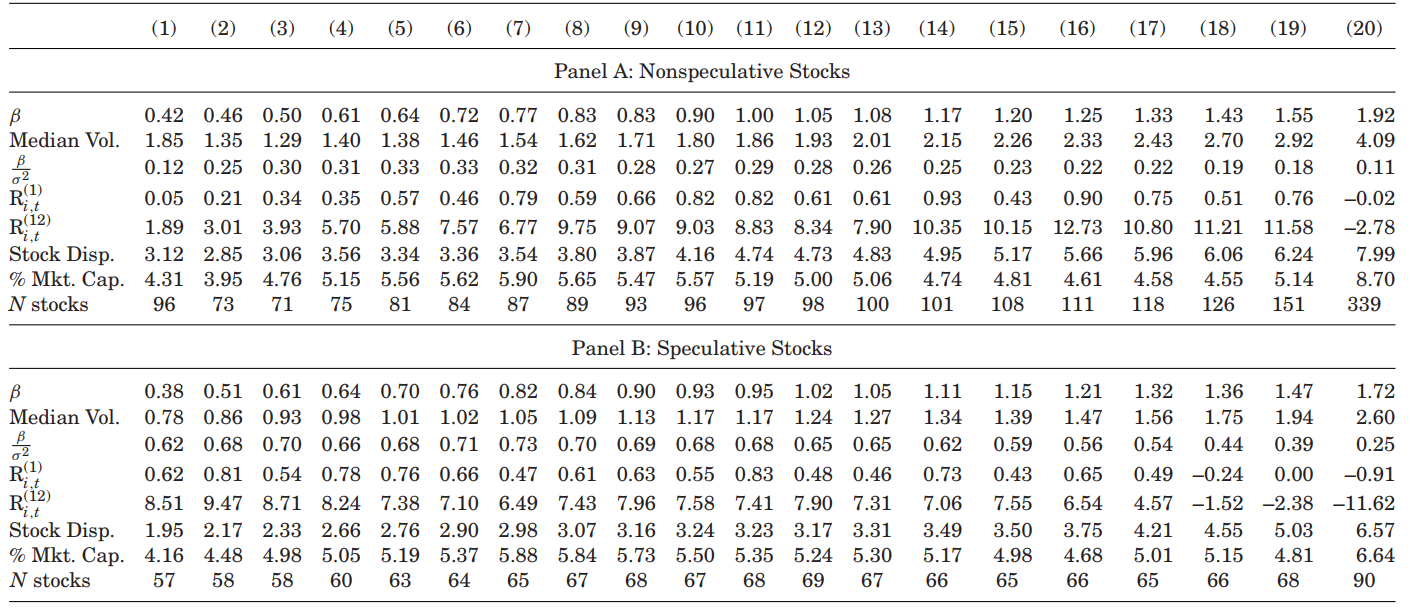
\includegraphics[width=0.8\linewidth]{"../Paper Presentaion/t3}
	\end{figure}
\end{frame}

\begin{frame}{$ \beta $-Sorted Portfolios}
	\begin{itemize}
		\item Rank stocks based on preranking ratio of $ \beta $ to $ \sigma^2 $ and define as speculative stocks all stocks with a ratio above  the  median ratio
		\item Then, within each of these two groups creat 10 $ \beta $-sorted portfolios
	\end{itemize}
	

			\begin{table}[htbp]
			\centering
			\resizebox{0.7\textwidth}{!}{
				\begin{tabular}{lcccccccccc}
	\toprule
	& 1     & 2     & 3     & 4     & 5     & 6     & 7     & 8     & 9     & 10 \\
	\midrule
	& \multicolumn{10}{c}{Nonspeculative} \\
	\midrule
	
	$\beta$  & 0.69  & 0.74  & 0.71  & 0.62  & 0.84  & 0.73  & 0.91  & 1.19  & 1.16  & 1.30 \\
	\multicolumn{1}{l}{12Return} & 50.07 & 42.39 & 53.00 & 59.10 & 64.57 & 43.80 & 55.05 & 71.15 & 57.46 & 56.05 \\
	\multicolumn{1}{l}{Mreturn} & 3.42  & 2.45  & 3.79  & 3.64  & 4.65  & 2.67  & 3.73  & 4.81  & 3.71  & 3.26 \\
	\multicolumn{1}{l}{Size} & 17    & 18    & 18    & 18    & 18    & 19    & 19    & 19    & 18    & 18 \\
	\midrule
	& \multicolumn{10}{c}{Speculative} \\
	\midrule
	$\beta$  & 0.69  & 0.91  & 0.90  & 1.10  & 1.14  & 1.05  & 1.26  & 1.24  & 1.40  & 1.58 \\
	\multicolumn{1}{l}{12Return} & 43.47 & 70.68 & 58.81 & 42.64 & 50.55 & 65.41 & 64.54 & 48.93 & 53.07 & 70.40 \\
	\multicolumn{1}{l}{Mreturn} & 3.07  & 4.91  & 4.23  & 2.42  & 3.23  & 4.38  & 3.95  & 3.24  & 3.43  & 4.75 \\
	\multicolumn{1}{l}{Size} & 18    & 18    & 19    & 19    & 19    & 19    & 19    & 19    & 19    & 19 \\
	
	\bottomrule
	
	
\end{tabular}%
				\label{tab:addlabel2}	
			}
		\end{table}
		  
\end{frame}

\begin{frame}{Speculative /Non Speculative}
	\begin{columns}
		\column{0.5\textwidth}
			\begin{figure}
			\centering
			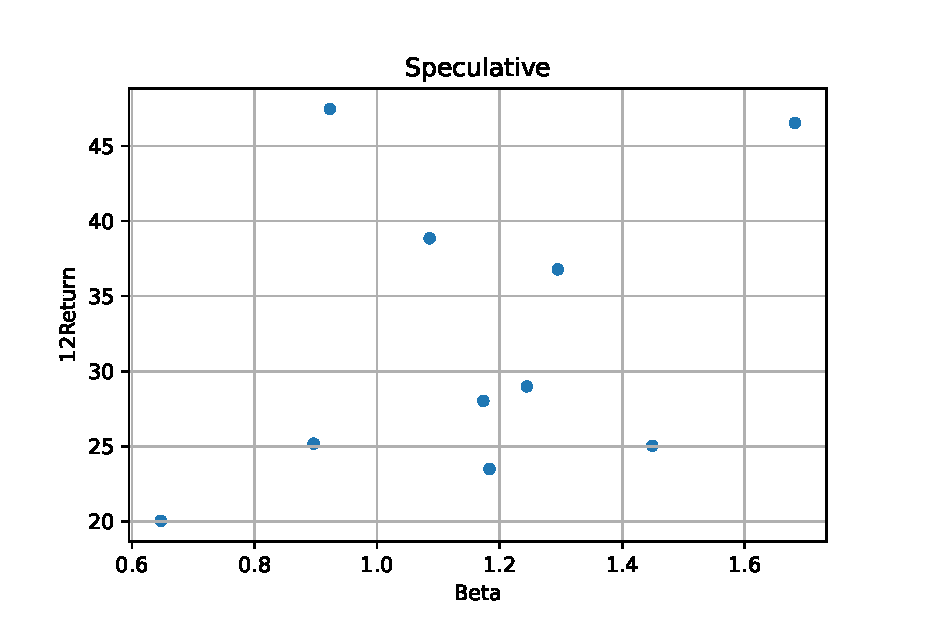
\includegraphics[width=\linewidth]{SpeculativeBetaReturn10.eps}
			\label{fig:SpeculativeBetaReturn10}
		\end{figure}
		\column{0.5\textwidth}
		\begin{figure}
			\centering
			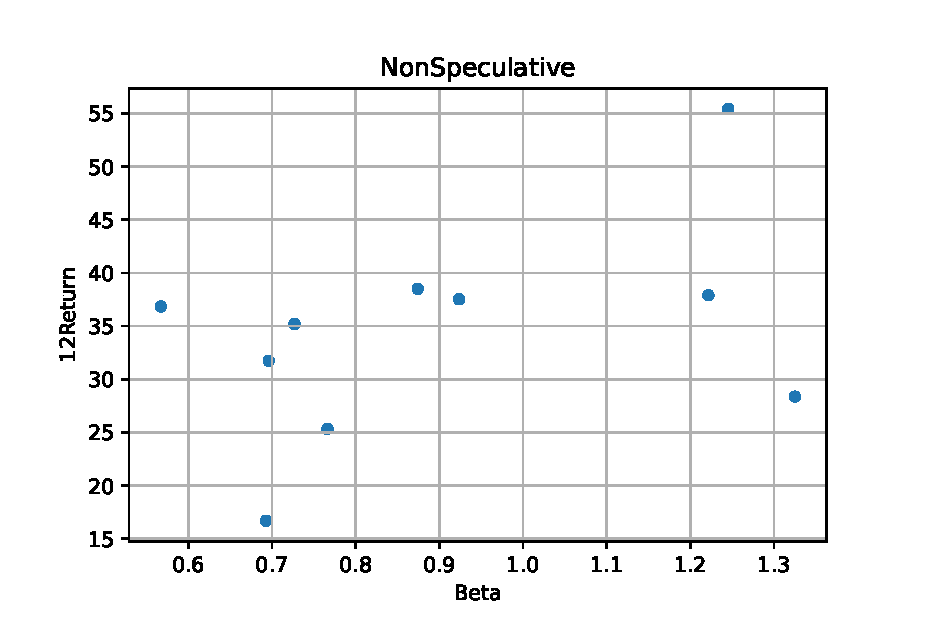
\includegraphics[width=\linewidth]{NonSpeculativeBetaReturn10.eps}
			\label{fig:NonSpeculativeBetaReturn10}
		\end{figure}
	\end{columns}
\end{frame}


\begin{frame}{Speculative /Non Speculative}
	\begin{figure}
		\centering
		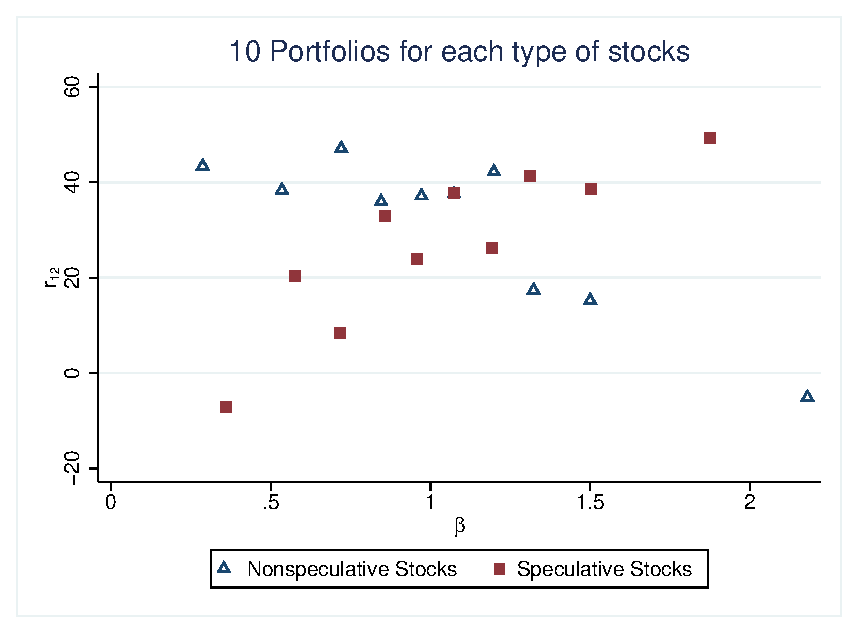
\includegraphics[width=0.7\linewidth]{10Sportfo.eps}
		\label{fig:speculativebetareturn}
	\end{figure}
	
\end{frame}



\end{document}